%=====================================================================
\section{The sharp successor distance}\label{sec:successor}
%=====================================================================
\begin{theorem}[Successor distance]\label{thm:successor}
For every $n\ge1$, $2\le\dist(n,n+1)\le6$. Moreover $\dist(163,164)=6$. Hence
\[
\sup_{n\ge1}\dist(n,n+1)=6.
\]
\end{theorem}
\noindent\emph{Source.} The bound, the nine path identities and the computation at $n=163$ are from U1-BND~\cite{u1bnd}; they are re-derived and re-checked here.
The lower bound $\ge2$ is Corollary~\ref{cor:nonadj}. We prove the upper bound by nine parametric routes (Subsection~\ref{ssec:nine}) and the sharpness by a ball certificate (Subsection~\ref{ssec:sharp6}).

\subsection{Nine path identities}\label{ssec:nine}
Table~\ref{tab:succ} lists the nine families. Class A, for instance, is $n=4t+1$ ($t\ge1$) with the four moves $+(4t+1),\,-2t,\,+t,\,-(2t+1)$.

\begin{table}[ht]\centering\small
\begin{tabular}{@{}cllcl@{}}\toprule
class & $n$ & range & moves & labels $N_1,\dots,N_\ell$ (sign $+$ forward, $-$ inverse)\\\midrule
A & $4 t + 1$ & $t\ge 1$ & 4 & $+(4 t + 1),\ -(2 t),\ +(t),\ -(2 t + 1)$ \\
B & $8 t$ & $t\ge 1$ & 5 & $+2,\ +2,\ -8,\ +(4 t),\ -(8 t + 1)$ \\
C & $8 t + 2$ & $t\ge 0$ & 5 & $+2,\ +(4 t + 1),\ +2,\ -8,\ -(8 t + 3)$ \\
D & $8 t + 4$ & $t\ge 0$ & 5 & $+2,\ +2,\ -8,\ +(2 \left(2 t + 1\right)),\ -(8 t + 5)$ \\
E & $8 t + 6$ & $t\ge 0$ & 5 & $+2,\ +(4 t + 3),\ +2,\ -8,\ -(8 t + 7)$ \\
F & $24 t + 3$ & $t\ge 1$ & 4 & $+(8 t + 1),\ -(4 t),\ +(3 t),\ -(6 t + 1)$ \\
G & $8 t + 7$ & $t\ge 0$ & 6 & $+(8 t + 7),\ +(t + 1),\ +(t + 1),\ -(2 t + 3),\ -(2 t + 3),\ -(2 \left(t + 1\right))$ \\
H & $24 t + 11$ & $t\ge 0$ & 6 & $+(24 t + 11),\ +24,\ -(2 \left(25 t + 12\right)),\ +(25 t + 12),\ -(25 \left(2 t + 1\right)),\ -4$ \\
I & $24 t + 19$ & $t\ge 0$ & 6 & $+1,\ +(24 t + 19),\ -3,\ -(3 \left(4 t + 3\right)),\ +(4 t + 3),\ -(6 t + 5)$ \\
\bottomrule\end{tabular}

\caption{The nine classes of the successor identity: $n=Mt+r$ with the stated range of $t$, and the labels of the route from $n$ to $n+1$. Moduli: $4$ for A, $8$ for B--E and G, $24$ for F, H, I.}\label{tab:succ}\end{table}

\begin{example}[Class A, in full]\label{ex:A}
Let $n=4t+1$, so $n+1=2(2t+1)$. The route and its cofactors:
\begin{align*}
4t+1 &\xrightarrow{\,+(4t+1)\,,\ c=1\,} (4t+2)^2=4(2t+1)^2 \\
&\xrightarrow{\,-2t\,,\ c=4\,} 4\cdot 2t=8t \\
&\xrightarrow{\,+t\,,\ c=8\,} 8(t+1)^2 \\
&\xrightarrow{\,-(2t+1)\,,\ c=2\,} 2\cdot(2t+1)=n+1.
\end{align*}
Each step is a legal move because the current state equals $c\,N$ (forward) or $c\,(N+1)^2$ (inverse): $4t+1=1\cdot(4t+1)$; $4(2t+1)^2=4\,(2t+1)^2$ with $N+1=2t+1$; $8t=8\cdot t$; $8(t+1)^2=2\,(2t+2)^2$ with $N+1=2t+2$. The first step is the universal edge $n\sim(n+1)^2$ (take $k=1$ in Definition~\ref{def:G}).
\end{example}

\begin{example}[Class G, in full]\label{ex:G}
Let $n=8t+7$, so $n+1=8(t+1)$. The six moves and states are
\begin{align*}
8t+7&\xrightarrow{+(8t+7)}64(t+1)^2 \xrightarrow{+(t+1)} 64(t+1)(t+2)^2\xrightarrow{+(t+1)}64(t+2)^4\\
&\xrightarrow{-(2t+3)}16(t+2)^2(2t+3)\xrightarrow{-(2t+3)}4(2t+3)^2\xrightarrow{-2(t+1)}8(t+1)=n+1,
\end{align*}
with cofactors $1,\ 64(t+1),\ 64(t+2)^2,\ 16(t+2)^2,\ 4(2t+3),\ 4$. For example in the fourth step $N+1=2t+4=2(t+2)$, $(N+1)^2=4(t+2)^2$ and $64(t+2)^4=16(t+2)^2\cdot4(t+2)^2$.
\end{example}

For all nine classes the states, labels and cofactors are listed in Appendix~\ref{app:succ}. The reader who wishes to check a class by hand has only to multiply each cofactor by the stated factor. The existence of such identities is not obvious from the form of the graph; they were found by computer search over parametric families of states, and what is proved here is that they are \emph{correct}, not that they are canonical (they need not be the shortest routes for individual $n$).

\begin{proposition}[Nine identities]\label{prop:nine}
For each class of Table~\ref{tab:succ} and every $t\ge t_0$ the displayed labels form a legal route from $n$ to $n+1$ with $\ell\le6$ moves. \emph{(Certified, Lemma~\ref{lem:certificate}.)}
\end{proposition}
\begin{proof} For each class the states $s_i(t)$ and cofactors $c_i(t)$ of Appendix~\ref{app:succ} satisfy the identities of Definition~\ref{def:param} (polynomial division, checked symbolically), their coefficients after the shift $t\mapsto t_0+u$ are non-negative with positive constant term, and $s_\ell=n+1$. Lemma~\ref{lem:certificate} gives legality for all $t\ge t_0$. \end{proof}

\begin{lemma}[Coverage]\label{lem:cover}
Every integer $n\ge1$ lies in a class of Table~\ref{tab:succ} with $t\ge t_0$, except $n=1$ and $n=3$. For these, $1\to4\to18\to81\to8\to2$ (moves $+1,+2,+2,-8,-1$) and $3\to16\to4$ (moves $+3,-1$) are routes of length $5$ and $2$.
\end{lemma}
\begin{proof} If $n$ is even, then $n\equiv0,2,4,6\pmod8$ lie in B, C, D, E ($n=8t$ needs $t\ge1$, which holds as $n\ge1$). If $n\equiv7\pmod 8$ it is in G. If $n\equiv1\pmod4$, it is in A for $t\ge1$ (all $n\ge5$), leaving $n=1$. If $n\equiv3\pmod8$ then $n\bmod24\in\{3,11,19\}$: classes F, H, I; class F requires $t\ge1$, leaving only $n=3$. The two exceptional routes are checked move by move: $1\cdot4=4$; $4=2\cdot2\Rightarrow18$; $18=9\cdot2\Rightarrow81$; $81=(8+1)^2\Rightarrow8$; $8=2\cdot(1+1)^2\Rightarrow2$; and $3\Rightarrow16=4\cdot4$, $16=4\cdot(1+1)^2\Rightarrow4$. \end{proof}
\emph{Proof of the upper bound in Theorem~\ref{thm:successor}.} Lemma~\ref{lem:cover} and Proposition~\ref{prop:nine}. \hfill$\square$

\subsection{Sharpness: $\dist(163,164)=6$}\label{ssec:sharp6}
\begin{proposition}\label{prop:163}
$\dist(163,164)=6$.
\end{proposition}
\begin{proof}
The upper bound is class I with $n=163=24\cdot6+19$, $t=6$: the route $163\xrightarrow{+1}652\xrightarrow{+163}107584\xrightarrow{-3}20172\xrightarrow{-81}243\xrightarrow{+27}7056\xrightarrow{-41}164$ (Figure~\ref{fig:worked}; the labels are $+1,+163,-3,-3(4t+3)=-81,+(4t+3)=+27,-(6t+5)=-41$).
For the lower bound, enumerate $\Ball_3(163)$ and $\Ball_2(164)$ by Theorem~\ref{thm:degree}: they have $874$ and $123$ vertices and are disjoint (\emph{computed}). By Lemma~\ref{lem:mitm} with $t=5$, $\dist(163,164)>5$.
\end{proof}
This completes Theorem~\ref{thm:successor}. The values $211$ and $283$ give the next instances; in the range $n\le2500$ the exact distance $6$ occurs for $41$ values of $n$, all of them $\equiv19\pmod{24}$ (computed here); the earlier release reports, for $n\le13500$, $262$ values with $\dist=6$ lying in the classes $11$ and $19$ modulo $24$ (inherited).
\begin{remark}[Attainment]
The supremum $6$ is attained at $n=163$, $211$, $283$, \dots; the identities of length six are upper bounds, and for many $n$ in the same residue class a shorter route exists. The precise statement is $\max_n\dist(n,n+1)=6$.
\end{remark}

\subsection{Distribution}
For $n\le2500$ the exact distances (computed here by the ball method) take the values $2,3,4,5,6$ with multiplicities $2,\ 21,\ 1545,\ 891,\ 41$ and mean $4.379$; $\dist(n,n+1)=2$ only for $n=3$ and $n=8$. The residue class of $n$ modulo $24$ does not determine the distance, only an upper bound (Figure~\ref{fig:dist}); but it is visible that the mean distance depends on the class.
\begin{figure}[ht]\centering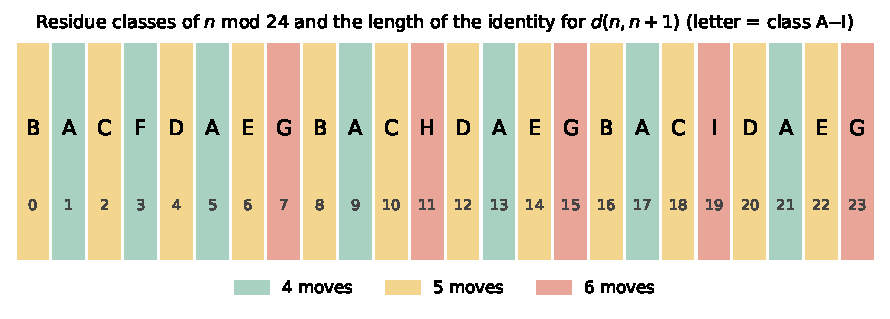
\includegraphics[width=.95\textwidth]{../figures/fig4_residue_map.pdf}
\caption{Residue classes modulo $24$ and the length of the corresponding identity for $\dist(n,n+1)$. Class letters are those of Table~\ref{tab:succ}.}\end{figure}
\begin{figure}[ht]\centering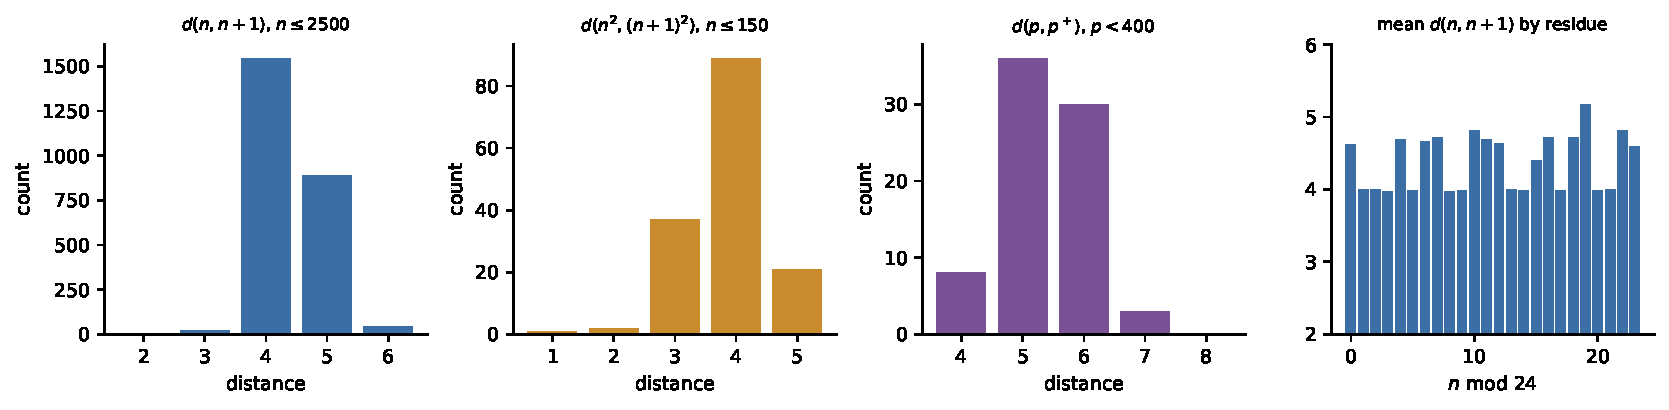
\includegraphics[width=\textwidth]{../figures/fig5_distributions.pdf}
\caption{Exact distances for consecutive integers ($n\le2500$), consecutive squares ($n\le150$) and consecutive primes below $400$ (computed), and the mean successor distance by residue class modulo $24$.}\label{fig:dist}\end{figure}
\begin{figure}[ht]\centering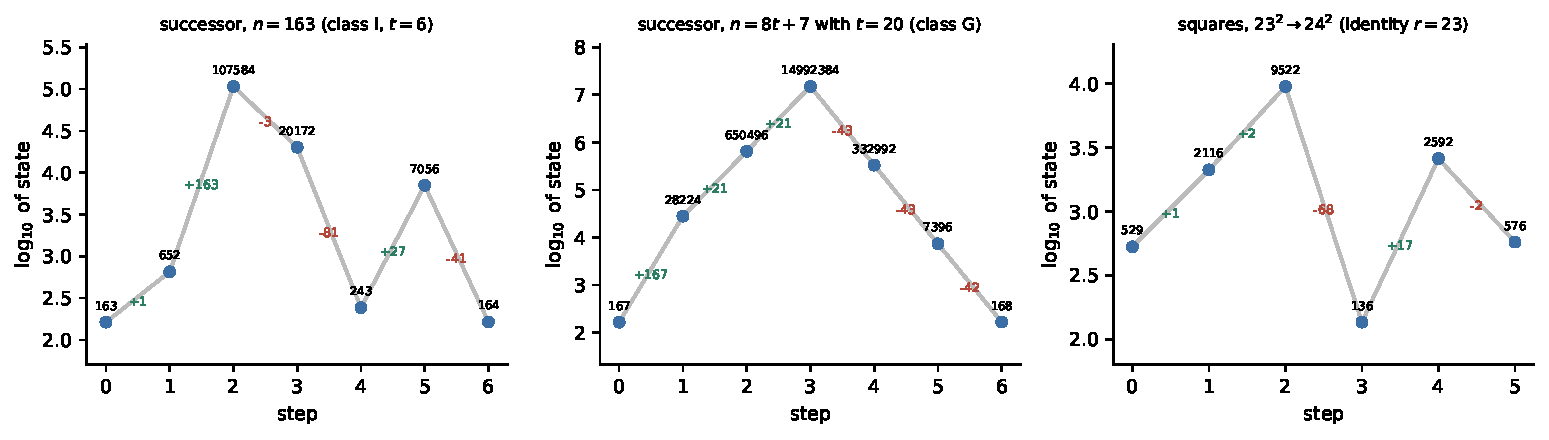
\includegraphics[width=\textwidth]{../figures/fig6_worked_paths.pdf}
\caption{Routes generated by the identities, on a logarithmic scale of the current state: class I at $n=163$ (the sharp instance), class G at $n=167$, and the square identity $r=23$ for $23^2\to24^2$. Green: forward moves, red: inverse moves. Every route rises to a power of $n$ and returns; this is the common shape.}\label{fig:worked}\end{figure}

\subsection{Connectivity and a Lipschitz bound}
\begin{theorem}[Connectivity]\label{thm:connected}
$G$ is connected, and $\dist(m,n)\le6\,|m-n|$ for all $m,n\ge1$.
\end{theorem}
\noindent\emph{Source.} The theorem follows from the successor bound of U1-BND~\cite{u1bnd}; the deduction is given here.
\begin{proof} For $m<n$ concatenate the routes $m\to m+1\to\dots\to n$ of Theorem~\ref{thm:successor}; the length is at most $6(n-m)$. \end{proof}
The bound $6|m-n|$ is a Lipschitz inequality from the integer line to $(G,\dist)$; it is far from sharp for distant arguments, as Corollary~\ref{cor:log} below shows.
\begin{corollary}[Cumulative form]
$\sum_{n=1}^{K}\dist(n,n+1)\le6K$, and a walk visiting $1,2,3,\dots,K+1$ in order, using geodesics between consecutive integers, has at most $6K$ edges.
\end{corollary}

%=====================================================================
\section{Multiplicative geometry: scaling, products and powers}\label{sec:mult}
%=====================================================================
\begin{theorem}[Scaling]\label{thm:scaling}
If $\{x,y\}\in E(G)$ then $\{mx,my\}\in E(G)$ for every $m\ge1$, with the same label. Consequently $\dist(ma,mb)\le\dist(a,b)$ for all $a,b,m\ge1$: multiplication by $m$ is a $1$-Lipschitz (non-expanding) map of $(G,\dist)$ into itself.
\end{theorem}
\noindent\emph{Source.} The scaling property is stated in U2-SQ~\cite{u2sq}.
\begin{proof} If $x=kN$, $y=k(N+1)^2$ then $mx=(mk)N$ and $my=(mk)(N+1)^2$. Apply this to every edge of a shortest path from $a$ to $b$. \end{proof}
The map $x\mapsto mx$ is injective but need not preserve distance; only the inequality $\le$ is claimed.
\begin{corollary}[Local steps by divisors]\label{cor:divstep}
If $m\mid x$ then $\dist(x,x+m)\le\dist(x/m,\,x/m+1)\le6$. In particular $\dist(x,x+1)\le6$ and $\dist(x,2x)\le5$ (take $m=x$ and use Theorem~\ref{thm:doubling}).
\end{corollary}

\begin{theorem}[Product inequality]\label{thm:product}
For all $a,a',b,b'\ge1$: $\ \dist(ab,a'b')\le\dist(a,a')+\dist(b,b')$.
\end{theorem}
\begin{proof} Scaling by $b$ gives $\dist(ab,a'b)\le\dist(a,a')$ and scaling by $a'$ gives $\dist(a'b,a'b')\le\dist(b,b')$. Use the triangle inequality. \end{proof}

\begin{theorem}[Power lifting]\label{thm:lifting}
For $k\ge1$ and all $x,y$: $\ \dist(x^k,y^k)\le k\,\dist(x,y)$. If $\{x,y\}$ is an edge with label $N$ and $x<y$, then $x^k,\,x^{k-1}y,\,\dots,\,y^k$ is a path of $k$ edges in which every step is the move $+N$; for $x>y$ the same sequence is traversed with every step the move $-N$.
\end{theorem}
\begin{proof} Consecutive terms are $mx$ and $my$ with $m=x^{k-j-1}y^j$; by Theorem~\ref{thm:scaling} this is an edge with the same label $N$ as $\{x,y\}$, traversed in the same direction (the larger endpoint is the one that is a multiple of $(N+1)^2$). Hence $\dist(x^k,y^k)\le k$ if $x\sim y$. For general $x,y$ apply this along a shortest path $x=v_0,\dots,v_d=y$: $\dist(x^k,y^k)\le\sum_i\dist(v_{i-1}^k,v_i^k)\le kd$. \end{proof}
\begin{figure}[ht]\centering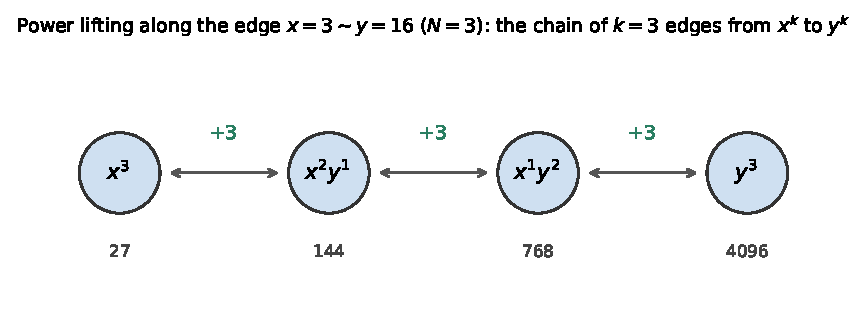
\includegraphics[width=.85\textwidth]{../figures/fig7_power_lifting.pdf}
\caption{Power lifting for the edge $3\sim16$ (label $N=3$, cofactor $1$) and $k=3$: $27\to144\to768\to4096$, each step the move $+3$.}\end{figure}
\begin{corollary}\label{cor:powers}
$\dist(n^k,(n+1)^k)\le6k$ for all $n,k\ge1$.
\end{corollary}
\noindent\emph{Source.} Power lifting and the bound $6k$ are stated in U2-SQ~\cite{u2sq}.
\begin{remark}
For $k=2$ Corollary~\ref{cor:powers} gives $12$, whereas Theorem~\ref{thm:squares} below gives the sharp value $5$: lifting is a general but not a sharp tool. For general $k$ the lifting bound $6k$ is linear in $k$; the sharp value is determined for $k=1$ (Theorem~\ref{thm:successor}) and $k=2$ (Theorem~\ref{thm:squares}).
\end{remark}

\subsection{Doubling and multiples}
\begin{theorem}[Doubling]\label{thm:doubling}
$\dist(n,2n)\le5$ for every $n\ge1$, and $\dist(1,2)=5$. Hence $\sup_n\dist(n,2n)=5$.
\end{theorem}
\noindent\emph{Source.} The doubling bound and its sharpness are from U2-001~\cite{u2}.
\begin{proof} The path $1\xrightarrow{+1}4\xrightarrow{+2}18\xrightarrow{+2}81\xrightarrow{-8}8\xrightarrow{-1}2$ has length $5$ (cofactors $1,2,9,1,2$: $1=1\cdot1$, $4=2\cdot2$, $18=9\cdot2$, $81=1\cdot9^2$, $8=2\cdot2^2$). Hence $\dist(1,2)\le5$ and by Theorem~\ref{thm:scaling} $\dist(n,2n)\le5$. For the lower bound, $\Ball_2(1)=\{1,4,16,18,25\}$ and $\Ball_2(2)=\{2,8,9,32,36,48,50,81,100\}$ are disjoint (\emph{computed}; each is easy to list by hand from Theorem~\ref{thm:degree}), so $\dist(1,2)>4$ by Lemma~\ref{lem:mitm}. \end{proof}
The balls are easy to list by hand from Theorem~\ref{thm:degree}: $\Nbr(1)=\{4\}$, $\Nbr(4)=\{1,16,18,25\}$; and $\Nbr(2)=\{8,9\}$, $\Nbr(8)=\{2,32,36,50,81\}$, $\Nbr(9)=\{2,36,48,100\}$.

\begin{table}[ht]\centering\small
\begin{tabular}{@{}l*{11}{c}@{}}\toprule
$j$ & 2&3&4&5&6&7&8&9&10&11&12\\\midrule
$\dist(1,j)$ & 5&3&1&5&5&4&4&4&4&6&4\\\bottomrule\end{tabular}
\caption{Exact distances $\dist(1,j)$ (computed). By scaling, $\dist(n,jn)\le\dist(1,j)$ for every $n$.}\label{tab:multiples}\end{table}
\begin{corollary}[Multiples]\label{cor:multiples}
$\dist(n,jn)\le\dist(1,j)$ for all $n,j\ge1$. In particular $\dist(n,4n)=1$, $\dist(n,3n)\le3$ and $\dist(n,11n)\le6$.
\end{corollary}

\begin{corollary}[Logarithmic distance from $1$]\label{cor:log}
For $n\ge1$ with binary expansion of length $\lambda$ and $\nu$ ones, $\dist(1,n)\le5(\lambda-1)+6(\nu-1)\le11\lfloor\log_2n\rfloor$. Consequently $\dist(m,n)\le22\log_2\max(m,n)$ for all $m,n\ge2$, so any set $\{1,\dots,N\}$ has diameter $O(\log N)$ in $(G,\dist)$.
\end{corollary}
\begin{proof} Build $n$ from $1$ by reading its binary digits from the top: doubling the current value $a$ costs at most $5$ by Theorem~\ref{thm:doubling} and Theorem~\ref{thm:scaling}; adding $1$ to an even value $a$ costs at most $6$ by Corollary~\ref{cor:divstep} (with $m=1$) and Theorem~\ref{thm:successor}. There are $\lambda-1$ doublings and $\nu-1$ additions. For $m,n$ pass through $1$. \end{proof}
This is a genuine metric statement: although consecutive integers can be at distance $6$ and arguments far apart are connected by routes of length linear in their difference (Theorem~\ref{thm:connected}), the graph distance grows at most logarithmically in the size of the integers. The constant $22$ is not optimised.
